\begin{frame}
	\frametitle{第四讲、数列极限的性质与判敛}
	\linespread{1.5}
	\begin{enumerate}
	  \item {\bf 内容与要求}{\color{blue}( \S2.2 )}
	  \begin{itemize}
	    \item 熟练掌握数列极限的基本性质
	    \item 熟练掌握数列收敛的判定方法
	  \vspace{1em}
	  \end{itemize}
	  \item {\bf 课后练习:}
	  \begin{itemize}
	    \item 书面作业:{\b 习题2.2:1(4,6),2(3),3,7,9,11}
	    \item 思考题:{\b 习题2.2:6,8,10,12}
	  \end{itemize}
	\end{enumerate}
\end{frame}

\section{复习与回顾}

\begin{frame}{数列极限的概念}
	\linespread{1.2}
	\begin{enumerate}
	  \item {$\limn a_n=a$}\pause $\Leftrightarrow{\b \forall\e>0,\exists
	  N,\forall n>N,|a_n-a|<\e}$
	  \uncover<9->{\item 反面:\alert{$\exists\e_0>0,\forall N,\exists
	  n_0>N,|a_{n_0}-a|\geq \e_0$}}
	\end{enumerate}
	\pause
	\begin{center}
		\resizebox{!}{4.8cm}{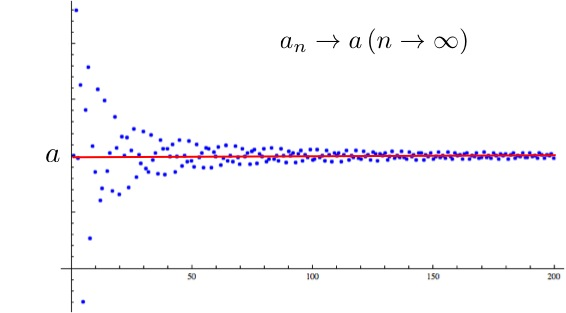
\includegraphics{./images/ch2/lim-en/en0.jpg}}
	\end{center}
	\pause
	\vspace{-5.66cm}
	\begin{center}
		\resizebox{!}{4.8cm}{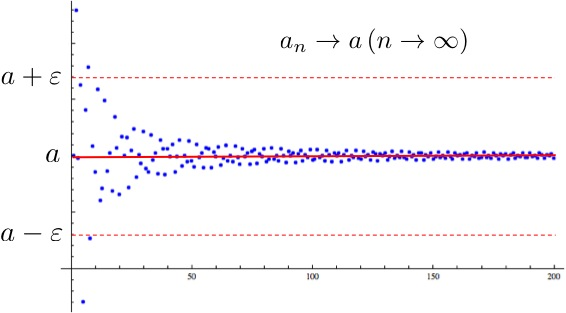
\includegraphics{./images/ch2/lim-en/en1.jpg}}
	\end{center}
	\pause
	\vspace{-5.66cm}
	\begin{center}
		\resizebox{!}{4.8cm}{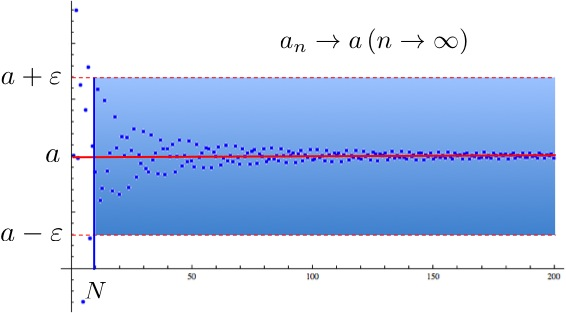
\includegraphics{./images/ch2/lim-en/en2.jpg}}
	\end{center}
	\pause
	\vspace{-5.66cm}
	\begin{center}
		\resizebox{!}{4.8cm}{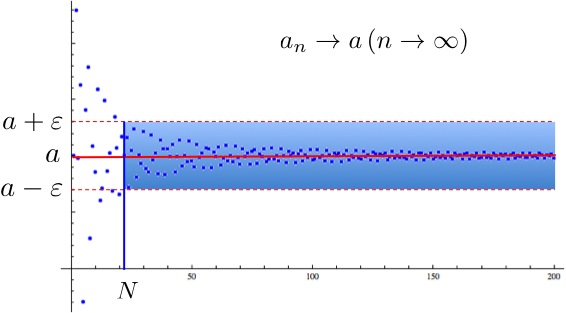
\includegraphics{./images/ch2/lim-en/en3.jpg}}
	\end{center}
	\pause
	\vspace{-5.66cm}
	\begin{center}
		\resizebox{!}{4.8cm}{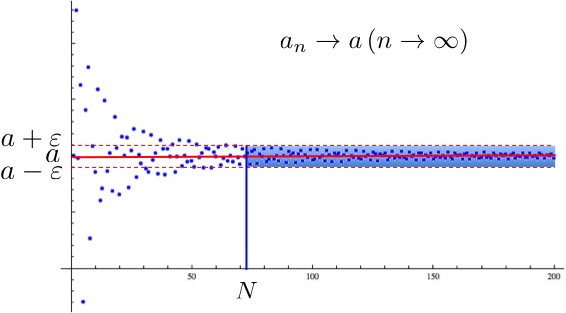
\includegraphics{./images/ch2/lim-en/en4.jpg}}
	\end{center}
	\pause
	\vspace{-5.66cm}
	\begin{center}
		\resizebox{!}{4.8cm}{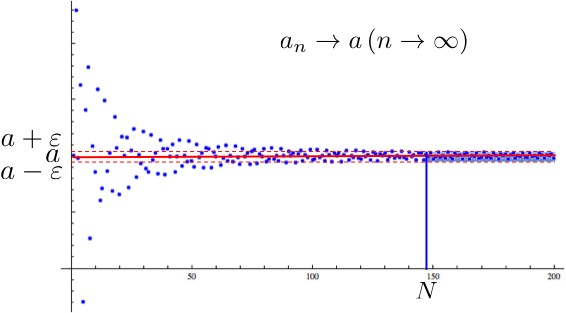
\includegraphics{./images/ch2/lim-en/en5.jpg}}
	\end{center}
\end{frame}

\begin{frame}{数列极限的基本性质}
	\linespread{1.5}
	\begin{enumerate}\pause 
	  \item {\bf 唯一性}\pause 
	  \begin{itemize}
	    \item 若$a,b$同为$\{a_n\}$的极限,则$a=b$\pause
	  \end{itemize}
	  \item {\bf 有界性}\pause 
	  \begin{itemize}
	    \item 若$\{a_n\}$收敛,则$\{a_n|n\in\mathbb{N}\}$有界\pause
	  \end{itemize}
	  \item {\bf 保号性}\pause 
	  \item {\bf 极限的四则运算}
	\end{enumerate}
\end{frame}

% \section{极限的性质(续)}
% 
% \begin{frame}{保号性}
% 	\linespread{1.4}\pause 
% 	\begin{block}{{\bf 定理2.1.3}\hfill P53}\pause 
% 		设$\lim\limits_{n\to\infty}a_n>0$,\pause 则有$N>0$,\pause 对任意$n>N$,$a_n>0$
% 	\end{block}\pause 
% 	\begin{block}{{\bf 推论}\hfill P54}\pause 
% 		\begin{enumerate}
% 		  \item 设对任意$n\in\mathbb{N}$,$a_n\geq
% 		  0$,\pause $\lim\limits_{n\to\infty}a_n=a$,\pause 则$a\geq 0$\pause 
% 		  \item 设$\lim\limits_{n\to\infty}a_n=a\ne
% 		  0$,\pause 则存在$N$,当$n>N$时,$|a_n|>|a|/2$\pause 
% 		  \item
% 		  设$\lim\limits_{n\to\infty}a_n=a$,\pause 且最多有有限个$a_n$小于零,\pause 则$a\geq 0$
% 		\end{enumerate}	
% 	\end{block}
% \end{frame}
% 
% \begin{frame}{极限的四则运算}
% 	\linespread{1.4}\pause 
% 	\begin{block}{{\bf 定理2.2.1}\hfill P57}\pause 
% 		设数列$\{a_n\},\{b_n\}$分别以$a,b\,(b\ne 0)$为极限,\pause 则
% 		\begin{enumerate}
% 		  \item $\lim\limits_{n\to\infty}(a_n\pm b_n)=a\pm b$\pause 
% 		  \item $\lim\limits_{n\to\infty}a_nb_n=ab$\pause 
% 		  \item
% 		  $\lim\limits_{n\to\infty}\displaystyle\frac{a_n}{b_n}=\displaystyle\frac{a}{\,b\,}$
% 		\end{enumerate}
% 	\end{block}\pause 
% 	\begin{exampleblock}{{\bf 例1:}计算极限\hfill P58-例2}
% 		$$\limn\df{2n^6+3n^4-n+10}{n^6+n^4+1}$$
% 	\end{exampleblock}
% \end{frame}
% 
% \begin{frame}
% 	\linespread{2}\pause 
% 	\begin{exampleblock}{{\bf 例2}\hfill P58-例1}
% 		设$\limn(a_n+b_n)=1$,$\limn(a_n-b_n)=3$,证明$\{a_n\},\{b_n\}$收敛,并求其值。
% 	\end{exampleblock}\pause 
% 	\vspace{2em}
% 	\begin{exampleblock}{{\bf 例3}\hfill P59-例3}
% 		设$q$为常数,且$|q|>1$,证明$\limn q^n$不存在
% 	\end{exampleblock}
% \end{frame}

\section{极限收敛的判定方法}

\begin{frame}{极限收敛的判定}
	\linespread{1.5}
	\begin{enumerate}\pause 
	  \item {\bf 子数列的收敛性}\pause 
	  \item {\bf 夹逼定理}\pause 
	  \item {\bf 单调有界原理}\pause 
	  \item {\bf 递推数列的判敛}
	\end{enumerate}
\end{frame}

\begin{frame}{子数列的收敛性}
	\linespread{1.5}\pause 
	\centerline{\large $\{a_{n_k}\}\pause
	:\,a_{n_1},a_{n_2},\ldots,a_{n_k},\ldots$}\pause 
	\begin{block}{{\bf 定理2.2.2}\hfill P59}\pause 
		数列收敛,当且仅当其任意子数列收敛,且极限相同。
	\end{block}\pause 
	{\ba{反面说法:}}{\b 若存在不收敛的子列,或存在极限不相同的子列,则数列不收敛。}\pause 
 	\vspace{1ex}
	\begin{block}{{\bf 定理2.2.3}(拉链定理)\hfill P60}
		数列$\{a_n\}$收敛,当且仅当$\{a_{2n}\}$和$\{a_{2n-1}\}$收敛于相同的极限。
	\end{block}
\end{frame}

\begin{frame}
	\linespread{1.2}\pause 
	\begin{exampleblock}{{\bf 课后思考}\hfill }
		已知数列$\{a_n\}$单调递增,它的一个子列$\{a_{n_k}\}$收敛于$a$,证明:$\limn a_n=a$。
	\end{exampleblock}
	\bigskip
	\pause 
	\ba{注:}$\{a_{n_k}\}$收敛于$a$的定义:\pause $\forall \e>0$,\pause $\exists
	\alert{K}$,\pause $\forall \alert{k>K}$,\pause 有 $$|a_{\alert{{n_k}}}-a|<\e,$$
	\pause 记为
	$$\lim\limits_{\alert{k\to\infty}}a_{n_k}=a\quad\pause \mbox{或}\quad a_{n_k}\to
	a\;\alert{(k\to\infty)}$$
\end{frame}

\begin{frame}{夹逼定理(迫敛定理)}
	\linespread{1.2}\pause 
	\begin{block}{{\bf 定理2.2.4}\hfill P60}
		设对任意$n\in\mathbb{N}$,$x_n\le a_n\le y_n$,且$\{x_n\},\{y_n\}$收敛于相同的极限
		$a$,则$\limn a_n=a$。
	\end{block}
	\pause 
	\begin{center}
		\resizebox{!}{4.5cm}{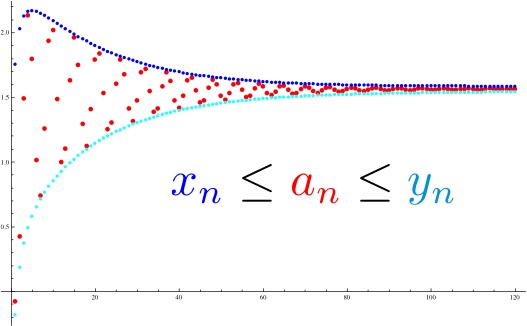
\includegraphics{./images/ch2/xay_n.jpg}}
	\end{center}
\end{frame}

\begin{frame}
	\linespread{1.5}
	\begin{exampleblock}{{\bf 例1}\hfill P61-例5}
		证明$\limn [(n+1)^k-{n}^k]=0$,其中$0<k<1$。
	\end{exampleblock}
	\pause 
	\vspace{1em}
	\begin{exampleblock}{{\bf 例2}\hfill P61-例6}
		设$a>0$为常数,证明$\limn \sqrt[n]{a}=1$。
	\end{exampleblock}
	{\ba{思考题:}}证明$\sqrt[n]n\to 1\,(n\to\infty)$
\end{frame}

\begin{frame}{单调有界原理}
	\linespread{1.2}\pause 
	\begin{block}{{\bf 定理2.2.5}\hfill P62}
		单调有界的数列必收敛。
	\end{block}
	\pause 
	\vspace{1em}
	\begin{alertblock}{{\bf 重要极限}\hfill P63-例7}
		$$a_n=\left(1+\df{1}{n}\right)^n\to e\quad (n\to\infty)$$
	\end{alertblock}
	\pause
	\begin{itemize}
	  \item $\{a_n\}$单调递增,$e$为其上确界
	\end{itemize}
\end{frame}

\begin{frame}{递推数列的收敛性}
	\linespread{1.4}\pause 
	\begin{exampleblock}{{\bf 例3}\hfill 分级考试题}
		已知$a_1,a_2$为常数,数列$\{a_n\}$满足:
		$$a_n=\df 12({a_{n-1}+a_{n-2}})\quad(n>2).$$
		证明$\{a_n\}$收敛,并求其极限。
	\end{exampleblock}
\end{frame}

\begin{frame}{递推数列的收敛性}
	\linespread{1.5}
	\begin{exampleblock}{{\bf 例4}\hfill P65-例9}
		设$a_1>0$,$a_{n+1}=\df 12\left(a_n+\df 1{a_n}\right)\,(n=1,2,\ldots)$,证明
		$\{a_n\}$收敛,并求其极限。
	\end{exampleblock}
	\pause
	\alert{\bf 注:}{\b 在已知极限存在的情况下},可通过在递推式两边同时取极限,然后解方程求得极限的值
\end{frame}

\begin{frame}
	\linespread{2}
	\begin{exampleblock}{{\bf 例5:}计算下列极限\hfill }\pause
		\begin{enumerate}
		  \item $\limn\df{n^2}{a^n}\quad (a>1)$\pause
		  \item $\limn\df{n!}{n^n}$\pause
		  \item
		  $\limn\underbrace{\sqrt{c+\sqrt{c+\ldots+\sqrt{c}}}}_{n\mbox{\small
		  个根号}}$\pause
% 		  \item $\limn\df{\cos^n\theta-\sin^n\theta}{\cos^n\theta+\sin^n\theta}\quad
% 		  (0\leq\theta\leq\df{\pi}{2})$
% 		  \item $\limn\left(1-\df 1{2^2}\right)\left(1-\df 1{3^2}\right)\ldots\left(1-\df 1{n^2}\right)$
		\end{enumerate}
	\end{exampleblock}
	\ba{注:}若极限存在,可由通项公式反推递推式,然后解方程求得极限值
\end{frame}

\section{特殊的极限计算方法}

\begin{frame}{特殊的极限计算方法}
	\linespread{1.2}\pause
	\begin{block}{\bf Stolz定理}
		设数列$\{y_n\}$满足$\limn\df 1{y_n}=0$,且$\{y_n\}$至少从某一项开始保持严格单调递增,
		则对任意数列$\{x_n\}$,若$\limn\df{x_n-x_{n-1}}{y_n-y_{n-1}}$存在,则必有
		$$\limn\df{x_n}{y_n}=\limn\df{x_n-x_{n-1}}{y_n-y_{n-1}}$$
	\end{block}
	\pause
	\alert{\bf 注:}Stolz定理主要用于计算"$\df{\infty}{\infty}$型"的极限
\end{frame}

\begin{frame}
	\linespread{1.2}
	\begin{block}{\bf 推论}
		若数列$\{a_n\}$收敛,则
		$$\limn\df{a_1+a_2+\ldots+a_n}{n}=\limn a_n$$
	\end{block}
	\pause
	\begin{exampleblock}{{\bf 例5:}计算以下极限}
		\begin{enumerate}
		  \item $\limn\df{1+\sqrt 2+\sqrt[3]{3}+\ldots+\sqrt[n]{n}}{n}$\pause 
		  \item $\limn\df{1^k+2^k+\ldots+n^k}{n^{k+1}},\quad(k\in\mathbb{N})$\pause 
		  \item $\limn\left(\df{1^k+2^k+\ldots+n^k}{n^{k}}-\df
		  n{k+1}\right),\quad(k\in\mathbb{N})$
		\end{enumerate}
	\end{exampleblock}
\end{frame}

\begin{frame}[<+->]{小结}
	\linespread{1.5}
	\begin{enumerate}
	  \item {\bf 数列极限的基本性质}
	  \begin{itemize}
	    \item 唯一性、有界性、保号性
	    \item 利用四则运算简化极限计算
	  \end{itemize}
	  \item {\bf 数列收敛的判定方法}
	  \begin{itemize}
	    \item 子数列、夹逼定理、单调有界原理
	    \item 递推数列
	  \end{itemize}
	\end{enumerate}
	\pause
% 	\vspace{1em}
	\pause
	\begin{exampleblock}{课后习题}
	  \begin{itemize}
	    \item 书面作业:{\b 习题2.2:1(4,6),2(3),3,7,9,11}
	    \item 思考题:{\b 习题2.2:6,8,10,12}
	  \end{itemize}
	\end{exampleblock}
\end{frame}

% \begin{frame}{课堂练习}
% 	\linespread{2}
% 	\begin{exampleblock}{{\bf 例6:}计算下列极限\hfill }
% 		\begin{enumerate}
% 		  \item $\limn\df{n^2}{a^n}\quad (a>1)$
% 		  \item $\limn\df{n!}{n^n}$
% 		  \item $\limn\df{\cos^n\theta-\sin^n\theta}{\cos^n\theta+\sin^n\theta}\quad
% 		  (0\leq\theta\leq\df{\pi}{2})$
% 		  \item $\limn\left(1-\df 1{2^2}\right)\left(1-\df 1{3^2}\right)\ldots\left(1-\df 1{n^2}\right)$
% 		\end{enumerate}
% 	\end{exampleblock}
% \end{frame}

\begin{frame}{课后思考}
	\linespread{1.5}
	\begin{exampleblock}{{\bf 例7}\hfill }
		设$0<a_1<2$,且$(2-a_n)a_{n+1}=1\,(n\in\mathbb{N})$,证明$\{a_n\}$收敛,求其极限。
	\end{exampleblock}
	\pause
	\begin{exampleblock}{{\bf 例8}\hfill }
		设$x_1=\df 12$,$x_{n+1}=x_n^2+x_n\,(n\in\mathbb{N})$,求
		$$\limn\left(\df 1{x_1+1}+\df 1{x_2+1}+\ldots+\df
		1{x_n+1}\right)$$
	\end{exampleblock}
\end{frame}

\begin{frame}{课后思考}
	\linespread{1.5}
	\begin{exampleblock}{{\bf 例9}\hfill }
		设$x_1=1$,$x_n=1+\df{x_{n-1}}{1+x_{n-1}}\,(n\geq 2)$,求$\limn x_n$。
	\end{exampleblock}
	\pause
	\begin{exampleblock}{{\bf 例10}\hfill }
		已知$0<x<1$,数列$\{a_n\}$定义如下:
		$$a_1=\df x2,\;a_n=\df x2-\df{a_{n-1}^2}2.$$
		证明$\{a_n\}$收敛,并求其极限。
	\end{exampleblock}
\end{frame}